\chapter{Methodology}

\section{Development Approach}
The development of Slotify followed a structured software engineering approach that combined requirement analysis, system design, implementation, and testing. The project was designed in phases so that each stage informed the next and helped maintain a clear path from concept to working system. This approach was important because the platform involves multiple user roles, booking workflows, and scheduling logic that must remain consistent across the system.

\begin{figure}[h]
\centering
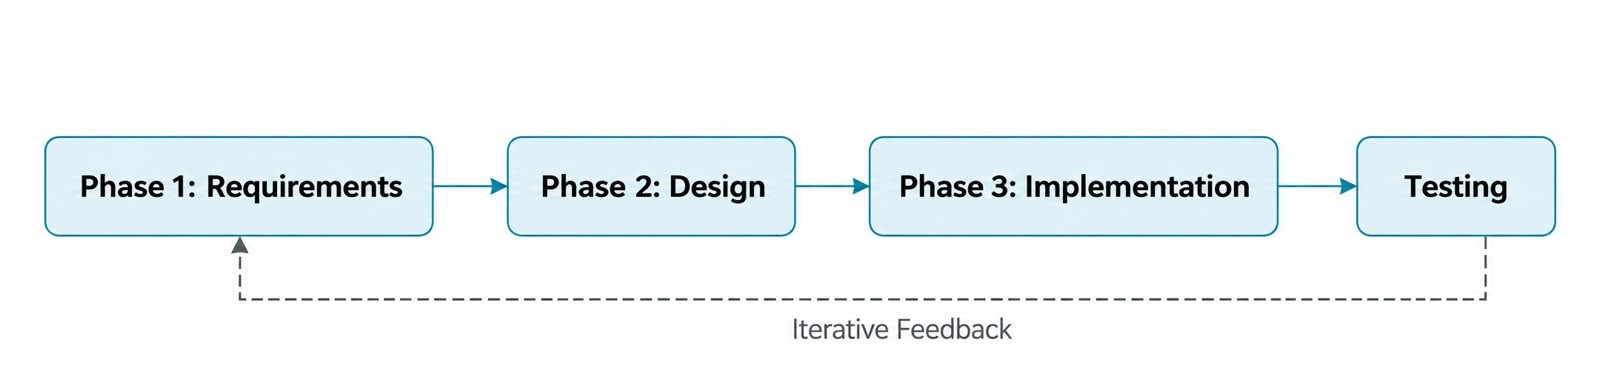
\includegraphics[width=0.9\textwidth]{images/figure 5-1.jpeg}
\caption{Methodology overview for the Slotify development lifecycle}
\end{figure}

\section{Phase 1: Requirements Gathering}
The first phase focused on identifying the core challenges faced by service-based businesses. This included understanding issues such as appointment conflicts, missed bookings, manual scheduling, and lack of business visibility. Input from the problem statement and literature review helped define the critical functional and non-functional requirements for the project.

\section{Phase 2: System Design}
Once the requirements were clear, the architecture and data model were designed to support multi-user scheduling. The design included a modular frontend, backend API layer, and database schema intended to handle business operations, service scheduling, and role-based access. The design phase also defined the flow of booking creation, confirmation, and reminder communication.

\section{Phase 3: Implementation}
The implementation phase involved building the backend logic, creating the frontend interfaces, and integrating the scheduling components. Core functionality such as slot generation, appointment validation, authentication, and notification services were implemented during this stage. The project was developed in a way that allowed real system operations to be tested with realistic booking scenarios.

\section{Phase 4: Testing}
Testing was carried out to validate that the application could create appointments correctly, prevent conflicts, and respond reliably under different conditions. This included checking the booking flow, verifying role access, and testing the reliability of slot calculation. The testing phase also helped identify issues related to concurrency and database constraints.

\section{Tools and Environment}
The project was developed using a modern web development stack to support scalability and maintainability. The frontend was built using React, while the backend used Node.js and Express. MongoDB was used for database storage, and email-based notifications were integrated through a transactional service. These tools were selected to support both the scheduling logic and the overall user experience.

\begin{table}[h]
\centering
\caption{Tools used during development}
\begin{tabular}{|p{3.5cm}|p{3.5cm}|p{5cm}|}
\hline
\textbf{Category} & \textbf{Tool} & \textbf{Purpose} \\
\hline
Version control & Git and GitHub & Source control and team collaboration \\
\hline
IDE & Visual Studio Code & Primary development environment \\
\hline
API testing & Postman & Endpoint testing and collection management \\
\hline
UI prototyping & Figma & Wireframes and layout planning \\
\hline
Database GUI & MongoDB Compass & Schema inspection and visual debugging \\
\hline
Frontend deployment & Vercel & Continuous deployment from GitHub \\
\hline
Backend deployment & Render & Node.js cloud hosting \\
\hline
Database hosting & MongoDB Atlas & Managed cloud database \\
\hline
\end{tabular}
\end{table}

\begin{table}[h]
\centering
\caption{Development phases and expected outputs}
\begin{tabular}{|p{3.5cm}|p{8cm}|}
\hline
\textbf{Phase} & \textbf{Outcome} \\
\hline
Requirements Gathering & Problem definition, business needs, and functional requirements identified \\
\hline
System Design & Architecture, database model, and workflow structure planned \\
\hline
Implementation & Frontend, backend, and scheduling logic developed \\
\hline
Testing & Appointment logic verified for reliability, conflict prevention, and correctness \\
\hline
\end{tabular}
\end{table}
